%
% chap003.tex
%

\chapter{Die Summe der ersten $n$ ungeraden natürlichen Zahlen}

Mit Hilfe von farbigen Edelsteinen lassen sich quadratische Muster
auch auf andere Weise erzeugen. Ein quadratischer Haken, der
sogenannte \textit{Gnomon}, mit andersfarbigen Steinen wird
um ein vorhandene Steinquadrat aus $m \cdots m$ gelegt.
Dafür werden $m + 1 + m$, d.h. $2m + 1$, Steine benötigt.
Das entspricht einer ungerade Anzahl von Steinen.

Ein paare einfache Beispiele:
\[
 \begin{array}{l}
  1 + 3 = 4 = 2^2 \\ 
  1 + 3 + 5 = 9 = 3^2 \\ 
  1 + 3 + 5 + 7 = 16 = 4^2 \\ 
  1 + 3 + 5 + 7 + 9 = 25 = 5^2 \\
  \dots
 \end{array}
\]

\textbf{Regel: Summe der ersten n ungeraden Zahlen}

Die Folge der ersten $n$ ungeraden natürlichen Zahlen
kann als quadratisches Muster von Winkelhaken
dargestellt werden.

Die Summe der ersten $n$ ungeraden natürlichen Zahlen
ist gleich der Quadratzahl $n^2$.
\begin{equation}
  1 + 3 + 5 + \dots + (2n - 1) = n^2
  \label{eq:formel_ungerade_natuerliche_zahlen}
\end{equation}

\begin{proof}[\textbf{Beweis durch vollständige Induktion}]
 $\text{}$
 
 \begin{itemize}
  \item Induktionsanfang: $n = 1$
        \[
         \sum_{i=1}^{1} (2\cdot 1 - 1) = 1 = 1^2
        \]
  \item Induktionsvoraussetzung:\\  
        Es gelte
        \[
         \sum_{i=1}^{n} (2i - 1) = n^2
        \]
  \item Induktionsschritt: $n = n + 1$
        \[
         \begin{array}{rcl}
           \sum\limits_{i=1}^{n+1} (2i -1)
           & = & \sum\limits_{i=1}^{n} (2i -1) + 2(n+1)-1 \\\\
           & = & n^2 + 2n + 1 \\\\
           & = & (n+1)^2
         \end{array}
        \]
 \end{itemize}
\end{proof}

\begin{example}Summe der ungeraden natürlichen Zahlen von $1$ bis $9$.
 
 Zur Lösung dieses Beispiels kann man entweder die oben genannte
 Formel verwenden:
 \[
  \sum_{i=1}^{5} (2i -1) = 5^2 = 25
 \]

 Oder man kann auch mit der Figur rechnen:
 
 \begin{figure}[H]
  \centering
  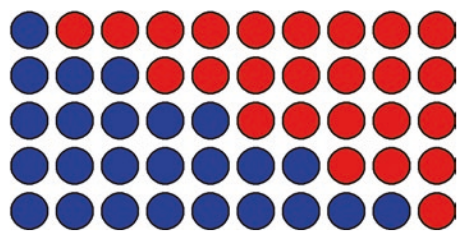
\includegraphics[width=.5\linewidth]{./images/muster03.png}
  \caption[]{Muster aus bunten Steinen zur Berechnung der Summe der ungeraden Zahlen $1,3,5,7,9$}
  \label{fig:muster_ungerade_1_bis_9}
\end{figure}

Zuerst legt man die blauen Steine in einer rechtwinkliger Dreicksform
von oben nach unten in aufsteigender Anzahl $1, 3, 5, 7, 9$ aus.
Danach verdoppelt man die Figur, indem man entsprechend viele rote Steine
von unten nach oben in absteigender Anzahl legt.
Als Resultat bekommt man eine Figure in Form eines Rechtecks.
Das Doppelte der Summe $1 + 3 + 5 + 7 + 9$ ist gleich $5\cdot 10 = 50$

Für die Summe $1 + 3 + 5 + 7 + 9$ ergibt sich der Wert $2\cdot 50 = 25$.
\end{example}
\vspace{.2cm}

\textbf{\textit{Aufgabe 2.5}:}
Begründen Sie: Eine weitere Möglichkeit der Herleitung der Formel
(\ref{eq:formel_ungerade_natuerliche_zahlen})
ergibt sich durch eine vielfache achsensymmetrische Anordnung von Steinen.

\begin{figure}[H]
  \centering
  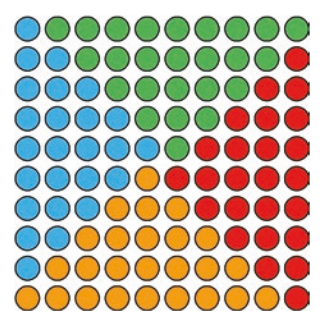
\includegraphics[width=.5\linewidth]{./images/muster04.png}
  \caption[]{}
  \label{fig:muster_ungerade_1_bis_9_achsensymmetrisch}
\end{figure}

\textbf{\textit{Lösung}:}
\[
  4 \cdot (1+3+5+7+9) = 8 \cdot (1+2+3+4+5) + 4\cdot 5
  = 8 \cdot \frac{1}{2}\cdot 4 \cdot 5 + 4 \cdot 5
  = 4 \cdot 4 \cdot 5 + 4 \cdot 5
  = 4^2 \cdot 5 + 4 \cdot 5
  = 4 \cdot 5^2
\]


